%\documentclass[12pt]{article}
\documentclass[espaco=simples,appendix=Name]{abnt}
\usepackage{abntex}
\usepackage[brazil]{babel}
\usepackage[T1]{fontenc}
\usepackage[utf-8]{inputenc}
\usepackage{hyperref}
\usepackage{times}
\usepackage{listings}
\usepackage[dvips]{graphicx}
\usepackage[num]{abntcite}      % citacoes do abntex
\usepackage{tabela-simbolos}    % tabelas de simbolos do abntex
\usepackage{dsfont}             % fonte
\usepackage{fancyvrb}

\citeoption{abnt-full-initials=yes}
\lstset{language=ruby,caption=Exemplo,label=Ruby, numbers=left, frame=single} 

\title{Expressividade da linguagem no ato de programar}

\author{Jônatas Davi Paganini}

\date{novembro de 2009}

\begin{document}
\maketitle
\begin{abstract}
Este trabalho busca mostrar uma linguagem de programação mais expressiva. Através de exemplos de programas de computador, será mostrado como a linguagem de programação pode ser simples e de fácil compreensão, como a linguagem Ruby pode ser caracterizada como uma linguagem de computador mais humana.

\textit{This paper shows how many expressive language is Ruby programming language. Through code examples, the language can be simple and easy to understand. This article shows how the computer's language can be like human's language.}

Palavras-chave: linguagem, expressividade, DSL, Ruby, código expressivo.
\end{abstract}

%\tableofcontents

\chapter{Introdução}

A construção de programas de computador retraí as pessoas, elas pensam que programas são complexos e difíceis de aprender. Com muitas regras e limites, a resistência ao aprendizado aumenta ainda mais. Em sua maioria, as linguagens oferecem suporte apenas em Língua Inglesa, tornando a interpretação da linguagem computacional ainda mais desafiante para o profissional. 

Os programas crescem e tornam-se complexos. Através de técnicas de desenvolvimento e o uso de uma linguagem bem específica, é possível mudar esta paisagem. Em uma análise das dificuldades que o programador encara, muitas vezes parte deste trabalho é culpa da linguagem, sua dificuldade de aprendizado e expressão.

Os tempos evoluiram e será abordada uma linguagem simples, com foco nas pessoas e não nos computadores. Com o objetivo de chegar mais próximo da realidade externa a um programa de computador, é possível escrever mini-linguagens, bibliotecas bem definidas com uma sintaxe única e expressiva para realizar o seu trabalho. Ferramentas específicas realizam tarefas específicas. Fazendo a escolha certa, é possível obter um código simples, que informe exatamente a sua funcionalidade, deixando a complexidade para camadas mais abstratas e específicas.  

Uma maneira inteligente de entender coisas complexas, é quebrá-las em partes menores. Quando um elemento demonstra-se complexo, pode ser dividido em outros conceitos e cada um deles terá sua responsabilidade mais específica e mais simples. Existem diversas maneiras de fragmentar um problema complexo, usando uma solução criativa, é possível diminuir a dificuldade de compreensão; estabelecendo terminologias, é possível desmassificar a complexidade.\cite{NazemiExpressiveCode}

Aplicando soluções simples, é possível fragmentar e unir um software complexo.


\chapter{A linguagem}


Linguagem não é somente as línguas, mas é uma série de outros sistemas de comunicação, notação ou cálculo, criados artificialmente pelo homem com objetivos específicos. Apesar de ser um código com regras determinadas, natural ou artificialmente, as linguagens podem ser consideradas, sob um ponto de vista comportamental, além de representarem ideias, comunicação, significados e pensamentos. \cite{linguagemLinguistica}. Embora os animais também se comuniquem, a linguagem propriamente dita pertence apenas ao Homem\cite{wikiLinguagem}.


Portanto, pode se dizer que as linguagens possuem flexibilidade e versatilidade, sendo usadas através do interesse e da vontade humana. Isso se deve à produtividade dos sistemas de linguagem, que possibilitam a construção e interpretação de novos sinais. Todos os sistemas possibilitam a seus usuários construir e compreender um número indefinido de enunciados, que jamais viram antes. Isso, por outro lado, se dá dentro dos limites estabelecidos pelas regras.

As linguagens de programação estão sob estes mesmos trilhos, conseguem ser flexíveis e estabelecer a definição de novos sinais e expressões. Este artigo abordará exemplos práticos de expressividade na programação, trará ao conhecimento do leitor uma forma produtiva de programar, analisando um domínio específico da linguagem (\textit{DSL - Domain Specified Language}), e as regras terminológicas que desenham as mini-linguagens que tornam o contexto expressivo.

As linguagens de computador têm o objetivo específico de traduzir o código para linguagem de máquina. Arquitetadas para facilitar o trabalho do homem, muitas vezes se tornam complexas e de difícil aprendizado. Devido a esta deficiência, são criadas ferramentas específicas para cada área do desenvolvimento. 

Ferramentas nascem com objetivo de minimizar o esforço humano. Para codificação, existem inúmeros \textit{Frameworks} que seguem este objetivo. Através da abstração de problemas comuns e adoção de soluções padronizadas, são desenhadas soluções que tornem o desenvolvimento de software produtivo.


\chapter{Evolução da linguagem de programação}

A evolução dos computadores trouxe dispositivos menores e mais potentes. Na década de 80, usavam-se grandes computadores para realizar pequenos processos, trinta anos mais tarde estes dispositivos ganharam velocidade, \textit{design} e consomem pouca energia. Dispositivos que cabem na palma da mão, com apenas alguns toques ou cliques, tornam acessível a informação desejada. 

Da mesma forma, os computadores ganharam potência, as linguagens de programação se tornaram expressivas e humanas. Tal dinamismo não tem o objetivo de trazer conforto à máquina, mas sim ao seu manipulador, o homem. 

A linguagem de computador, inicialmente era grosseira e de difícil compreensão, com o passar do tempo, as técnicas foram evoluindo, ganhando forma e expressão. Houve uma percepção de mudança, que tornaria a linguagem de programação uma auxiliadora do programador e não uma interpretadora.

Uma linguagem tem os seus limites, na maioria dos casos são formais e burocráticos. A linguagem Ruby quebra esta formalidade, torna o processo de codificação simples e livre. Em outras palavras, ela não bloqueia o trabalho do programador.

\section{Exemplo 'Hello world'}

   O programa Hello world é o programa mais conhecido no mundo inteiro e é o exemplo mais básico de uma linguagem de programação, com o objetivo de imprimir a mensagem "Hello, world!" e guiar o iniciante em sua primeira compilação/execução de um programa de computador. Abaixo seguem dois exemplos "Hello, world" em duas linguagens de programação distintas: asssembly e ruby.


\subsection {Exemplo usando a linguagem de programação \textit{assembly}}

\textit{Assembly} ou \textit{Assembler} é uma notação escrita por humanos que permite escrever instrução de máquina de forma mais fácil. \textit{Assembly} paga o preço da complexidade pelo reduzido número de comandos e opções.

\begin{lstlisting}[label=exemplo em assembly,caption=Exemplo em \textit{assembly}]
   variable:
      .message   db   "Hello world!\$"
   code:
      mov  ah,9
      mov  dx,offset .message
      int  0x21
      ret
\end{lstlisting}

Sem dificuldades, a listagem acima \ref{exemplo em assembly} demonstra-se complexa. Apenas para imprimir uma frase foram necessárias 6 linhas. Essa declaração não tão amigável é usada para realizar o mesmo objetivo do comanddo abaixo \ref{exemplo hello world ruby}, apenas estão escritas de forma diferente. O fato é que os compiladores exigem uma quantidade mínima de declarações para que possa compilar e executar.


\subsection {Exemplo usando a linguagem de programação \textit{ruby}}

\begin{lstlisting}[caption=Exemplo em \textit{ruby}]
   print "Hello, world!"
\end{lstlisting}

 \textit{Ruby} demonstra-se mais simples nestas exigências, é possível compilar apenas uma expressão, não precisando de declarações e nem padrões repetitivos. O código possui apenas o comando de impressão e a frase que deseja ser impressa.

\section { A simplicidade da linguagem }

Foi necessário apenas uma linha de código para representar o mesmo exemplo na linguagem \textit{ruby}. No exemplo mais simples, o objetivo é apenas imprimir "Hello, world!" e é exatamente isso que está escrito. Diferente de \textit{assembly}, \textit{ruby} não é uma linguagem compilada e, sim, dinâmica. Assim, tudo acontece em tempo real, enquanto está sendo executado.
   
\begin{lstlisting}[caption=Tradução do programa \textit{ruby}]
   imprima "Ola mundo!"
\end{lstlisting}

Apenas com uma linha de código é possível fazer exatamente o que está sendo proposto. Este programa de computador foi escrito de forma simples e humanamente legível, diferente da primeira instrução de máquina escrita em \textit{assembly}. Com poucas palavras, cumpriu exatamente o objetivo do software no domínio em questão.

Exemplos como este, mostram o poder do homem em categorizar e generalizar as informações. Desta forma, a percepção mudou de 'programar para o computador' para 'programar para as outras pessoas'. Anteriormente, com uma programação rígida e a escassez de processamento, a codificação de um software realmente fazia parte de um processo árduo e lento, em que não era possível tornar agradável a leitura de uma instrução de computador.

\section { A burocracia da linguagem }

Declarar e inicializar variáveis, importar pacotes, classes finais e fechadas são fatores que interferem no trivial desenvolvimento de software. As linguagens estáticas empurram o programador a escrever mais código, forçam a declarar estruturas sem sentido, por não saber lidar com o problema em 'alto nível'.

\begin{lstlisting}[label=HelloWorldJava, caption=Programa Hello World em Java]
 public class Hello {
     public static void main(String[] args) {
         System.out.println("Hello, World!");
     }
 }
\end{lstlisting}

Para ser possível executar um código em java, este deve estar em uma classe Java, em arquivo na extensão .java. A classe deve ser pública e deverá conter um método estático, sem retorno (\textbf{void}) com o nome \textbf{main}. Este método receberá como parâmetro um vetor de \textit{strings} que representam os parâmetros da linha de comando. Para compilar o arquivo java, será necessário usar o compilador \textbf{javac} que então criará um arquivo com o mesmo nome do código fonte, com a extensão .class. Esse arquivo pode ser executado usando o comando \textbf{java}. 

Todos estes passos devem ser seguidos sem falhas para que o exemplo "Hello, world!" seja compilado e executado usando a linguagem java. Cada detalhe deste tem um motivo e é importante em algum aspecto na linguagem. Mas, em muitos momentos, estes recursos se tornam desumanos e complexos, ofuscando a expressividade da linguagem.

\chapter { A linguagem \textit{ruby} }

\textit{Ruby} é uma linguagem dinâmica, \textit{open source}, com foco na simplicidade e produtividade. Tem uma sintaxe elegante, de leitura natural e fácil escrita. Com um grande número de bibliotecas disponíveis gratuitamente (gems), tem atraído muitos desenvolvedores.

Para usá-lo no \textit{MacOSX} ou \textit{Linux}, é necessário abrir o \textbf{Terminal} ou \textbf{Console} e, no Windows, pode-se usar o \textbf{Command-DOS} e, após, digitar \textbf{ruby.exe} para invocar o compilador, \textbf{irb} para iniciar uma interação.


\section { O compilador \textit{ruby} }

\textit{Ruby} é uma linguagem de \textit{script}, dinâmica e compila em tempo de execução. O mesmo compilador que compila o código também o executa. O compilador pode ser invocado usando a linha de comando e receber apenas um fragmento de código por parâmetro para compilar.

\begin{lstlisting}[caption=Usando o compilador na linha de comando]
jonatas@xonatax-mac:~$ ruby -e "puts 1+2"
3
\end{lstlisting}

Também é possível escrever um arquivo ou vários

\section { \textit{Ruby} Interativo - IRB }

Existe um programa chamado IRB, que vem instalado com compilador de \textit{ruby} e que serve para interagir com a linguagem na forma de console. As linhas do console \textit{ruby} digitadas são iniciadas por \textbf{>>} e as linhas que trazem o resultado da expressão são iniciadas por \textbf{=>}. Estes símbolos, quando exibidos no início da linha, não fazem parte do código de programação, apenas identificam a situação do terminal interativo.

\begin{lstlisting}[caption=Usando o compilador na linha de comando]
jonatas@xonatax-mac:~$ irb
>> 1.class
=> Fixnum
>> 1 + 2
=> 3
\end{lstlisting}

\section { Tipos de dados }

Tudo em \textit{ruby} é objeto, todas as classes são abertas e podem ser alteradas ou extendidas. A seguir, serão abordados os tipos básicos de dados para trabalhar com \textit{ruby}.

\subsection { \textit{Strings} }

As \textit{strings} podem ser limitadas por vários delimitadores, em geral, são usadas aspas simples e duplas, mas existem outras formas. Uma \textit{string} é um dado que contém uma informação em formato texto. Em \textit{ruby} é encarado como uma cadeia de caracteres, e pode ser também fácilmente manuseado como um vetor de caracteres.

\begin{lstlisting}[caption=Exemplos de uso de \textit{string}]
>> " outra string" + ' mais uma' + %[ outra ]
=> " outra string mais uma outra "
\end{lstlisting}

\subsection { Números }

Os números são objetos, como qualquer outro, e os operadores são simples métodos.

\begin{lstlisting}[caption=Exemplos de uso de números ]
>> 1.class
=> Fixnum
>> 1.class.ancestors
=> [Fixnum, Integer, Precision, Numeric, Comparable, Object, Kernel]
>> 1.0.class
=> Float
\end{lstlisting}

\subsection { \textit{Hashes} }

Este tipo de elemento amarzena valores como uma matriz, mas é possível acessar os valores através de uma chave. O valor do elemento é indicado a partir da expressão:

\begin{lstlisting}[caption=Syntaxe do hash]
{ :chave => valor }
\end{lstlisting}

Tanto chave quanto valor podem ser objetos de qualquer tipo. Lembrando que a chave é a forma de acessar um valor, logo não poderá haver chaves iguais na mesma estrutura. 

\begin{lstlisting}[label=exemplohash, caption=Exemplos de uso de hashes]
sexo = { "M" => "Masculino", "F" => "Feminino"}
sexo["M"] # => "Masculino"

pessoa = { :nome => "jonatas", :idade => 22, :cpf => "047..." }
pessoa[:rg] # => nil
\end{lstlisting}

Quando invocada uma chave que não existe, a expressão retorna \textbf{nil} ou \textbf{nulo}. \textbf{Nil} também é um objeto em \textit{Ruby} e é um objeto falso, o que auxilia no tratamento de excessões simples como requerir o documento de \textbf{cpf} ou \textbf{rg} da variável \textbf{pessoa} declarada acima\ref{exemplohash} :

\begin{lstlisting}[caption=Exemplos de uso de hashes com operador ou ]
documento = pessoa[:rg] || pessoa[:cpf] # => "047..."
print "sem documento!" if documento.nil?
\end{lstlisting}

No caso acima, quando não houver \textbf{rg}, irá buscar por \textbf{cpf} e atribuir a \textbf{documento}. Se não encontrar nenhum dos dois, então irá imprimir a mensagem avisando a falta do documento.

\subsection { Entrada de dados }

No exemplo abaixo, será feita uma pergunta para o usuário e, quando ele confirmar, a resposta irá saudar o usuário.

\begin{lstlisting}[caption=Exemplo de entrada de dados ]
 print "qual seu nome?"
 nome = gets
 print "oi #{nome}"
\end{lstlisting}
 
Na primeira linha, é impressa a pergunta. Na próxima linha, a variável \textbf{nome} recebe o valor digitado pelo usuário, que é captado através do comando \textbf{gets}.

Em seguinda, é impressa a saudação juntamente com a variável \textbf{nome}. O uso da interpolação \#\{\} embutido na string concatena o resultado da expressão interna invocando o método to\_s(transforma em \textit{string}).


\subsection { Métodos }

Os métodos podem ser usados a partir de uma classe ou estarão definidos na classe \textbf{Object} que é a classe maior. Métodos são formas de interagir com o ambiente atual e encapsulam a função com parâmetros. Eles podem pertencer às classes ou às instâncias. 

\begin{lstlisting}[caption=Exemplo de método ]
def ligar_para(telefone)
  puts "ligando para #{telefone}"
end
\end{lstlisting}

\subsection { Classes e Módulos }
 
Classe é a declaração que permite definir uma classe marcado pela palavra \textit{class}, seguida do nome de elementos. Após isso, vem o corpo com as definições do corpo. O fim do corpo é marcado pela palavra 'end'.

Módulos permitem dividir comportamentos de classe e de instância, permitindo assim a múltipla extensão de classes. Ele pode ser usado em blocos e sub-blocos e todo o código gerado fica encapsulado na declaração. Esse recurso também pode ser usado para agrupar classes do mesmo gênero. 

\begin{lstlisting}[caption=Exemplo de módulo ]
  module Mamifero
    def mamar
      print "mamando..."
    end
  end
  class Gato
    include Mamifero
    def miar
       print "meauuuu"
    end
  end
\end{lstlisting}

Os módulos também são uma boa possibilidade para criar espaços de nomes. Com este recurso, é possível trabalhar com nomes específicos e sem repetições.

No exemplo acima, é definido um módulo \textbf{Mamifero}, cujas características internas estão sendo declaradas. Um módulo não pode ser instanciado, ele é apenas usado como um espaço de nomes. O objetivo dele é organizar pequenos comportamentos que podem ser utilizados em outros momentos.

\begin{lstlisting}[caption=Exemplo de módulo como espaço ]
module Condominio
  include PortaoEletronico
  class Apartamento
   # ... define o apartamento internamente
  end
end 
\end{lstlisting}

\subsection{ Variáveis } 

Quando iniciados com apenas um arroba (@), indicam ser uma variável de instância. Diferente de Java e muitas outras linguagens, não é necessário declarar a variável antes de usá-la. Elas, simplesmente, criam a referência logo na primeira vez em que são usadas.

As variáveis locais são iniciadas por letras ou \textit{underscore}.

A atribuição de um valor a uma variável é feita através do sinal de igualdade (=).

\begin{lstlisting}[caption=Exemplo de variável local ]
meu_nome = "Jonatas"
\end{lstlisting}

A leitura da expressão acima seria: meu nome (a variável) é igual a Jonatas.

Em uma classe, as váriaveis são usadas como atributos internos.

\begin{lstlisting}[caption=Exemplo de variável de instância em uma classe ]
class Pessoa
  def initialize(nome)
    @nome = nome
  end
  def saudar
    puts "ola #{@nome}"
  end
end
\end{lstlisting}

O código anterior declarou a classe, que pode ser utilizada da seguinte forma:

\begin{lstlisting}[caption=Exemplo de utilização da classe descrita acima ]
jonatas = Pessoa.new "Jonatas"
jonatas.saudar 
\end{lstlisting}

\subsection { Blocos de código }

\cite{programmingRuby}
Segundo Dave Thomas, todo mundo já quiz implementar o seu próprio recheio de método na sua própria estrutura. Um bloco pode ficar entre chaves ou entre as palavras \textit{ do } e \textit{ end }.

\begin{lstlisting}[caption=Exemplo de bloco de código ]
   5.times { print "hello word" }
\end{lstlisting}

Traduzindo: 
\begin{lstlisting}[caption=Exemplo de bloco de código ]
   5.vezes { imprima "ola mundo" }
\end{lstlisting}

O bloco de código é extensamente utilizado em \textit{frameworks} para apenas criar a estrutura e tornar óbvio o objetivo da linguagem.


\chapter{ Shoes }

\section{O que é Shoes?}

\textit{Shoes} é um \textit{framework} para a construção de interfaces rápidas. \textit{Shoes} nasceu pra ser fácil. Realmente, feito para iniciantes absolutos. Com esta ferramenta, é realmente fácil de fazer interfaces e artes gráficas. 

Esta ferramenta permite criar interfaces \textit{desktop} para todas as plataformas e muitos divertidas de aprender.

\section{ Primeiro exemplo }

Este é um dos exemplos mais simples do \textit{shoes}. 

\begin{lstlisting}[caption=Primeiro exemplo do \textit{framework Shoes}  ]
Shoes.app { 
  button("Click me!") {
     alert("Good job.") 
  }
} 
\end{lstlisting}

Este programa foi escrito em uma linguagem chamada \textit{Ruby}. Consiste em uma janela com um botão. Quando o botão for clicado, ela deverá responder por: "\textit{Good job.}" ou seja "Bom trabalho."

\textit{Shoes} roda na maioria das plataformas operacionais. Isto é ótimo pois é possível escrever apenas uma vez e usar no \textit{Linux, MacOSX, Windows} e muitos outros.

%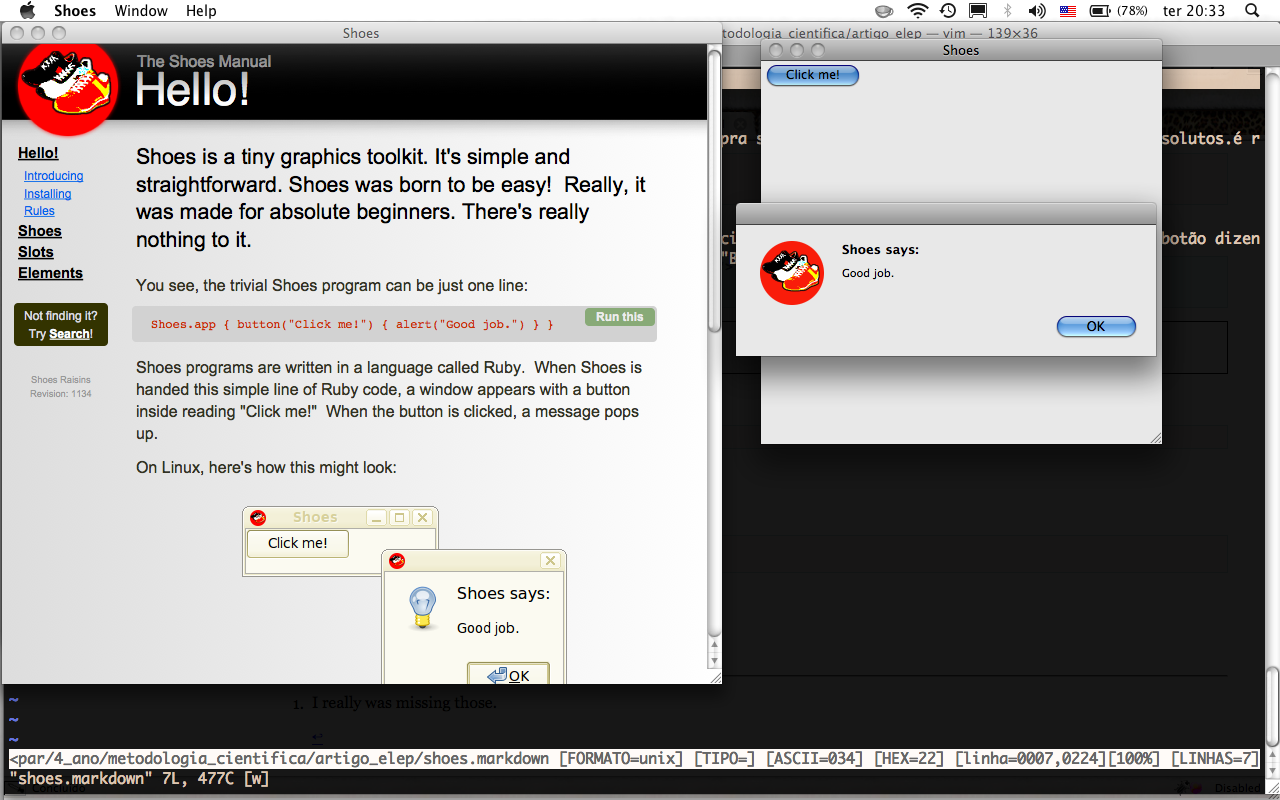
\includegraphics[scale=0.6]{shoes_hello_world.eps}
% (exemplo rodando no Mac OS X)!

\subsection{ Exemplo de expressividade - um bloco de notas com \textit{Shoes} }

Como próximo exemplo, será progamado um bloco de notas que possa apagar e inserir novas notas em uma janela. O programa será composto por:
\begin{itemize} 
  \item uma janela com um título "Minhas Notas", largura de 300 pixels. E dentro desta janela terá 
  \begin{itemize} 
    \item uma linha de edição para escrever a nota
    \item um botão para adicionar a anotação que quando for clicado deve 
    \begin{itemize} 
      \item adicionar o que foi escrito na linha de edição para as notas abaixo listadas
      \item limpar o texto da linha de edição da nota
    \end{itemize} 
  \end{itemize} 
  \item cada nota adicionada deve conter um link para remover a nota \ldots
\end{itemize} 


\subsection { Funcionamento do \textit{framework} }

Como descrito na primeira linha de código do exemplo anterior, o \textit{framework} é declarado, contendo uma janela principal. Esta janela, recebe um título e um tamanho inicial.

A declaração:

\lstinputlisting[caption=Um bloco de anotações com Shoes]{shoes_tarefas.rb} 

\textbf{Shoes.app} inicia um aplicativo do \textit{framework} e, dentro do corpo deste método, é possível empilhar e enfileirar objetos. Com suas definições específicas de janela, também pode receber parâmetros. Este objeto pode encaixar muitos outros componentes internamente. Também é possível manipular elementos de fora para dentro e de dentro para fora, fazendo com que um bloco interfira no outro, sem dificuldades.

Como o exemplo acima mostra, o \textit{framework Shoes} basicamente é uma pilha de componentes, podendo adicionar, empilhar e remover elementos com facilidade e clareza. Estes elementos, quando empilhados, podem interagir apenas empilhados, ou empilhados e aninhados a outras pilhas de elementos. 


\lstinputlisting[firstline=1, lastline=1, caption=Primeira explicação do \textit{framework Shoes}]{shoes_tarefas.rb} 

Estes parâmetros como \textbf{título \textit{(title)}} e \textbf{tamanho \textit{(width)}} são pertencentes à janela principal do aplicativo e podem ser acompanhados de outros, como bloqueio de redimensionamento de janela.

Os parâmetros no formato \textbf{chave} e \textbf{valor} facilitam o uso e a extensão das possibilidades para cada elemento. Infinitamente, podem trabalhar com novas funcionalidades e com os valores padrão.

Na segunda linha do código existe a declaração do elemento da interface edit\_line que é responsável pela linha de edição que permite a entrada de dados.
\lstinputlisting[firstline=2, lastline=2, caption=Entendendo a linha de edição]{shoes_tarefas.rb} 

Este método edit\_line retorna um componente do \textit{Shoes} do tipo 'caixa de entrada de texto', e é possível acessar o valor do texto digitado através do atributo \textbf{text}. 

\lstinputlisting[firstline=3, lastline=9, caption=Entendendo o botão e sua ação]{shoes_tarefas.rb} 

No fragmento acima, é declarado o botão que faz. Muito semelhante à especificação do programa \textit{Shoes} proposto, este fragmento cumpre a seguinte parte: 

\begin{itemize} 
  \item adicionar o que foi escrito na linha de edição para as notas (linhas 5 e 6)
  \item cada nota adicionada deve conter um link para apagar a nota (linha 6)
  \item limpar o texto da linha de edição da nota (linha 8) \ldots
\end{itemize} 

Traduzindo, literalmente, a declaração do botão:

\begin{lstlisting}[caption=Botão adicionar - código traduzido]
  botao "adicionar" {  
    @notas.adicionar { 
      paragrafo(@anotacao.texto + " " + 
          link("apagar") {|nota| nota.pai.remover })
    }  
    @anotacao.texto = ""
  } 
\end{lstlisting}

Um botão adicionar \textbf{(botao "adicionar")}, que faz com que o texto da anotação \textbf{(@anotacao.texto)} seja adicionado sob as notas \textbf{(@notas.adicionar)} já existentes. Quando clicado no link de apagar \textbf{(link("apagar"))} o elemento \textbf{(nota)}, este referencia-se ao seu 'pai' que o remove como 'filho' \textbf{(nota.pai.remover)}, desaparecendo da pilha de anotações \textbf{(@notas)}.

\lstinputlisting[firstline=10, lastline=10, caption=Entendendo a pilha de notas]{shoes_tarefas.rb} 

Traduzind, literalmente, a linha 10:

\begin{lstlisting}[caption=Entendendo a pilha de componentes]
  @notas = pilha :margem => 20, :largura => 300
\end{lstlisting}

A variável \textbf{@notas} é igual a uma pilha de componentes \textit{shoes} com margem de 20 pixels, e largura de 300 pixels. Essa pilha não exibe nada na tela até que não seja adicionado nenhum elemento nela. Quando o botão adicionar for pressionado, então ela é usada para adicionar o texto escrito na \textbf{nota}. Observe que foi usada a variável em um bloco de código, antes mesmo de ela existir. Se o botão for clicado antes da pilha de notas ser criada, então o sistema lançará uma merecida excessão. 

\textit{Shoes} trabalha com pilhas e fluxos (\texttt{ stacks and flows }), esse conceito permite empilhar elementos e criar fluxos com outros. Eles não se misturam, mas podem interagir. A pilha criada foi atribuida à váriavel \textbf{ @notas } e foi definido uma margem e uma largura para esta pilha de elementos. O processo pode funcionar recursivamente dentro desta pilha, permitindo criar o mesmo fluxo interno e concatenar elementos com liberdade.

\chapter { Linguagens de domínio específico }

No domínio específico de construir telas, o \textit{framework} tem características que ressaltam a sua expressividade. A simplicidade de fazer um botão ter uma ação é expressiva, no domínio de construir um botão com uma mensagem de alerta. É muito semelhante ao exemplo a seguir\ref{exemplo botao}. Se é um botão, consequentemente, terá uma mensagem e uma ação.  Em uma linha de edição (\textbf{edit\_line}), terá exatamente as propriedades de uma entrada de texto. 


\begin{lstlisting}[label=exemplo botao, caption=Simplicidade do botão]
botao("mensagem") { alerta("clicou no botao" } 
\end{lstlisting}


Para desenhar uma linguagem de domínio específico, deve-se olhar para a forma mais fácil de expressar-se naquele contexto.

Cada elemento, em seu domínio específico, tem a sua forma de expressão. Por exemplo,  existem várias opções para construir uma janela, esses elementos podem ser descritos através dos parâmetros do comando. Uma janela pode ter um título, um tamanho inicial, ser redimensionável, etc.

\begin{lstlisting}[label=exemplo janela, caption=Expressividade da construção de uma janela]
janela :largura => 300, :altura => 500, 
       :titulo => "Janela de exemplo" {

  botao("exemplo")
}
\end{lstlisting}


Cada problema, no seu contexto, pode ser expressivo quando usando uma terminologia adequada para o domínio específico. A maioria das linguagens de programação dificulta a criação desta sintaxe dentro da própria linguagem. \textit{Ruby} trabalha com estas linguagens de forma mais transparente. Leandro Heuert\cite{dslLeandro}, abordou o exemplo da criação de uma receita de bolo no seu domínio específico da seguinte forma: 

\begin{lstlisting}[label=exemplo receita, caption=Expressividade de uma receita no seu domínio específico\cite{dslLeandro}]
receita {
  nome "Bala de Pinga"
  ingrediente 1, 'kg', 'acucar cristal'
  ingrediente 1, 'copo', 'pinga'
  ingrediente 2, 'copos', 'agua'
  ingrediente 2, 'envelopes', 'gelatina incolor'
  ingrediente 1, 'envelopes', 'gelatina vermelha'
}
\end{lstlisting}

Os domínios específicos tornam o código estético e preciso. Yukihiro Matz Matsumoto, o criador da linguagem \textit{Ruby}, pergunta, em uma entrevista a Dave Thomas, se as linguagens influenciam o ser humano. Ele discute o que é uma boa linguagem de programação, que maneira muda sua forma de pensar e como o faz um programador melhor.

Como japônes, logo pensa em japônes, mas tem que traduzir para inglês a sua forma de pensar. Ele argumenta que não existe uma maneira de programar em japônes, a linguagem simplesmente não permite, essa não seria uma boa linguagem para explorar como uma linguagem de programação. As linguagens devem fazer você pensar melhor e faze-lo um melhor programador.\cite{programmingRuby}



Em outra entrevista \cite{entrevistaDivertidaComMatz} com Matz, Matsumoto comenta sobre a importância de aprender vários tipos de linguagem de programação. Para entender a produtividade que a linguagem pode oferecer, é necessário conhecer os bons aspectos das linguagens de \textit{script}, funcionais, lógicas, etc. Aprender linguagens é uma maneira de aprender a programar. Ler códigos fontes é uma maneira de obter conhecimento e informação. Também não deve-se dar foco às ferramentas, pois elas mudam. O importante é conhecer a base fundamental dos algorítmos.

Ser preguiçoso é uma fonte de inspiração para programar em \textit{Ruby}, as máquinas servem aos homens e a elas pertence o esforço. Falando pouco e se expressando bem, é possível comandar computadores com produtividade.

Heuert\cite{dslLeandro} conclui que, quanto mais conhecido é o domínio específico, melhor será a solução. Uma linguagem pode ser desenhada com sucesso para um determinado escopo, pode ser comunicativa para as pessoas e para os computadores e expressiva como os exemplos aqui apresentados.

A atividade de trabalhar com a linguagem, uma forma de se comunicar com a máquina, deve ser divertida e, em primeiro lugar, de homem para homem, depois, de homem para máquina e, por fim, de máquina para máquina\cite{entrevistaDivertidaComMatz}. Em outras palavras, deve iniciar por uma definição compreensiva ao homem, depois deve ser comunicado para a máquina de forma fácil e, finalmente, a máquina pode compreender e se preocupar com suas tarefas de máquina.


Com uma linguagem bem desenhada, como Heuert citou "pode-se facilmente que pessoas que tenham um mínimo necessário de conhecimento em linguagens de programação consigam entender o quê está acontecendo por trás de um software"\cite{dslLeandro}. Trabalhando com elementos conhecidos na contexto do programador, é possível que, mesmo sendo um iniciante, codifique sem dificuldades, já que conhece o domínio específico.

Existe um framework muito utilizado pelos programadores \textit{ruby}, chamado \textit{ActiveRecord}. Este \textit{framework} tem o objetivo de encapsular o mapeamento objeto-relacional que permite a persistência de objetos em banco de dados e conversão de um registro de uma tabela para um objeto. O exemplo a seguir\ref{exemplo activerecord} faz uma busca por um usuário ativo do sistema que possua o \textit{login} igual a 'jonatas'.

\begin{lstlisting}[label=exemplo activerecord, caption=Exemplo de busca com o framework ActiveRecord]
User.active.find_by_login("jonatas")
\end{lstlisting}

Traduzindo na literal tem-se:
\begin{lstlisting}[label=exemplo activerecord traduzido, caption=Exemplo traduzido de busca com o framework ActiveRecord]
Usuario.ativo.busca_por_login("jonatas")
\end{lstlisting}

A expressão acima\ref{exemplo activerecord} irá executar uma consulta no banco de dados que fará o filtro necessário pelo login e por usuários ativos e trará o objeto instanciado se algum registro for encontrado. 
Com este \textit{framework} também é possível mapear relacionamentos entre outros objetos agregados.

\begin{lstlisting}[label=exemplo classe extendida activerecord, caption=Exemplo de classe extendida do ActiveRecord]
class NotaFiscal < ActiveRecord::Base
  validates_uniqueness_of :numero
  validates_presence_of :cliente

  belongs_to :cliente
  has_many :itens
end
\end{lstlisting}

Quando uma classe é estendida do \textit{framework ActiveRecord}, abre-se uma gama de métodos específicos para indicar os relacionamentos existentes, validar, filtrar, inserir, alterar atributos ou excluir. Também é possível criar observadores para diversos pontos e estados do objeto. Traduzindo a listagem anterior, tem-se a seguinte declaração:

\begin{lstlisting}[label=exemplo classe extendida activerecord traduzido, caption=Exemplo de classe do ActiveRecord traduzida]
class NotaFiscal < ActiveRecord::Base
  validar_unicidade_do :numero
  validar_presenca_do :cliente

  tem_muitos :produtos
  pertence_a :vendedor
end
\end{lstlisting}

Em um \textit{software} determinado, dá-se uma nota fiscal, que terá um número único, não permitirá ser lançada sem um cliente, terá muitos produtos e pertence a um vendedor. O exemplo acima apresenta dois tipos de métodos mapeadores das associações e os validadores.

A metaprogramação é o poder de estender a linguagem a partir da própria linguagem. Dave Thomas\cite{programmingRuby} ressalta que uma das coisas que mais chama atenção em \textit{Ruby} é a facilidade de instrospecção à linguagem. Com este recurso, é possível criar objetos dinamicamente, é possível trabalhar com o inesperado criando métodos e classes de forma dinâmica, através da própria linguagem. Também é este o recurso que mais auxilia na definição do domínio específico da linguagem a ser desenhada. 


\chapter {Considerações finais}

A programação de computadores é um trabalho árduo e de difícil compreensão. Mas, quando localizado em um domínio específico, pode-se apresentar simples e com fácil manutenção. A programação torna-se fácil, quando existe clareza nos objetivos e expressividade na linguagem escolhida. O conhecimento das regras e recursos da linguagem é crucial para obter resultados realmente expressivos. 

%Pode-se criar um mundo dentro de outro e torná-lo tão grande quanto o primeiro, tão preciso quanto o seu contexto e útil para seu usuário como um escravo incansável. Nesse momento existe a satisfação pelo trabalho executado.
A escolha das premissas e da terminologia no domínio específico não dependem apenas da escolha do programador, que irá arquitetar a solução, mas também dos recursos que a linguagem oferece. \textit{Ruby} destaca-se na simplicidade de programar, na facilidade de impôr limites e desenhar linguagens internamente. Com os recursos aqui exemplificados, é possível escolher boas ferramentas, codificar com expressividade, escolher nomes convenientes e criar códigos de máquina mais humanos.


\bibliographystyle{plainat}
\begin{thebibliography}{9} 
\bibitem{wikiLinguagem} 
Wikipédia, 
Acesso em setembro de 2009.

\url{http://pt.wikipedia.org/wiki/Linguagem}

\bibitem{programmingRuby} 
Thomas, D. 
Programming Ruby: The Pragmatic programmers’ Guide. 
Segunda edição. Dallas, Texas: The Pragmatic Bookshelf, 2006.

\bibitem{dslLeandro} 
HEUERT, L. 
Linguagens Específicas de Domínio: um exemplo prático em Ruby.
Francisco Beltrão: UNIPAR, 2008.

\bibitem{agileRails} 
Thomas, Dave; Hansson, David Heinemeier.
Agile Web Development with Rails 
Second Edition.  Dallas, Texas: The Pragmatic Bookshelf, 2007.

\bibitem{entrevistaDivertidaComMatz}
Ruby Creator Yukihiro Matsumoto.
Interview by Stephen Ibaraki, I.S.P.
\url{http://www.stephenibaraki.com/rubycreater122101.htm}
Acesso em novembro de 2009.

\bibitem{entrevistaAudioComMatz}
Matsumoto, Y.
Ruby Design Principles
Technometria with Phil Windley, 
Acesso em novembro de 2009.
%(Entrevista de audio em inglês). 
\url{http://itc.conversationsnetwork.org/shows/detail1638.html}

\bibitem{cantWriteAExpressiveCode}
Gageot, David.
We can’t write expressive code,
Acesso em novembro de 2009.
\url{http://blog.javabien.net/2009/01/12/can-we-really-write-expressive-code}

\bibitem{rubyPhilosophy}
Venners, B. The Philosophy of Ruby
A Conversation with Yukihiro Matsumoto
\url{http://www.artima.com/intv/ruby.html}
Acesso em novembro de 2009.

\bibitem{linguagemLinguistica}
Lyons, John.
Linguagem e Linguística,
Inglaterra: Universidade de Sussex, 1981.
% Tradução
% Marilda Winkler Averbug

\bibitem{NazemiExpressiveCode}
Nazemi, Kate.
Expressive Code
Massachusetts College of Art and Design, 2005.

\url{http://www.dynamicmediainstitute.org/projects/expressive-code}

\end{thebibliography} 

\end{document}


